\documentclass[../main.tex]{subfiles}
\begin{document}


In this chapter, we are interested in giving a review of the literature on how to build relational structures automatically. While reviewing pieces of work, we are interested in two aspects: one is the pipeline used to build the relational structure itself, which comprises the mathematical models and algorithms applied to this end, along with their assumptions. If these assumptions are met in our model, then their pipeline or a subset of it could be useful.
\par Additionally, the second aspect of interest are the goals and components of the target relational structure, i.e. the entities and relationships the authors modelled. Discovering links between pairs of bird species is different from segmenting vowel sounds in human speech, for example. Although these differences will probably be reflected in different pipelines, understanding them is key in order to produce a pipeline that will yield better results for our work.
\par However, limiting ourselves to works focusing exclusively on this task might be too restrictive: results from bird classification, clustering and detection could also prove useful for our project. For example, feature extraction is common to all tasks, and state-of-the-art feature extraction is mandatory in order to achieve better results. Therefore, whenever relevant, works on these tasks will also be cited in this review.
\par This chapter is presented as follows: firstly, a general overview of pipelines for building relational structures is given; afterwards, we present a review of feature extraction methods used in acoustic signals; algorithms for building relational structures are reviewed next; finally, a discussion on how the referenced methods are relevant a working pipeline for our scenario is presented.

\section{Relational structures and pipelines}\label{general_pipeline}
A relational structure is one that shows links between objects. In this work, we will assume these links to be a binary relations $R$ over a single set $X$, i.e. $R \subseteq X \times X$. One way of representing such relations is a square matrix $A$, called \emph{adjacency matrix}, such that $A \in \mathbb{R}^{n \times n}$, where $n =\left\vert{X}\right\vert$.
\par In real life, information about objects can be represented as a relational structure. As the number of objects grows large, specific subsets of $R$ may present an increasingly "complex" topology. "Complex graphs" (as they are commonly called in the literature) and how to identify them have been extensively discussed in the field. In \cite{Kim2008}, the authors give a narrowed definition for complex graph, which we adapt as follows:
\theoremstyle{definition}
\begin{definition}{Complex graph}. One such that its topological features deviate from random graphs. In other words, a graph that contains many different subgraphs.
\end{definition}
\par A problem that has attracted attention in recent years is community detection. Given a graph $G = (X, E)$ depicting a relation between pairs of objects in $X$, community detection can be seen as a problem of clustering over $X$, i.e. partitioning the vertices $X$ in such a way that the edges between those in different clusters "are comparatively fewer than those between those belonging to the same cluster" \cite{Fortunato2010}. 
\par Clustering is the task of "grouping or segmenting a collection of objects into subsets or clusters, such that those within each cluster are more closely related to one another than objects assigned to different clusters" \cite{hastie2008}. An example of clustering for the 2-dimensional case can be seen in \ref{clustering}.
\begin{figure}[h]
\centering
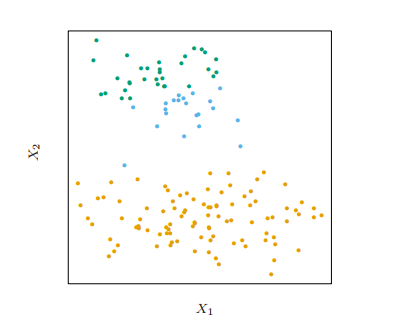
\includegraphics{clustering}
\caption{Simulated data in the plane, clustered into three classes. Image taken from \cite{hastie2008}.}
\label{clustering}
\end{figure}
\par Therefore, performing clustering requires computing the \emph{closeness} of elements in the set of objects $X$. Proximity, closeness, similarity or dissimilarity, all refer to \emph{distance functions} or \emph{measures}. 
\theoremstyle{definition}
\begin{definition}{Measure}.
A non-negative function $d$ satisfying:
\begin{enumerate}
\item Triangle inequality. $d(x, z) \leq d(x, y) + d(y, z) $
\item Symmetry. $d(x, y) = d(y, x)$
\item $d(x, x) = 0$
\item $d(x, y) = 0 \implies x = y$
\end{enumerate}
\end{definition}
\par Thus, defining a measure requires knowledge about what kind of objects we are grouping. In Machine Learning in particular, we will also be concerned by how we transform data into objects for which we can define a measure. This process, called \emph{feature extraction}, consists in "deriving features from raw data that can be used as input for a learning procedure" \cite{hastie2008}. The goal is to use domain knowledge to extract features that will reduce redundancy in raw data and highlight distinguishing characteristics, thus optimising the learning procedure in both, correctness and performance \cite{Bishop2006}. 
\par By working our way backwards, we have implicitly defined a general pipeline to be followed to build relational structures: the algorithms that do so, require the definition of a measure between objects. These objects will be the vectors or features extracted from each object of interest. A diagram depicting this procedure is shown in \ref{pipeline}.
\begin{figure}
\centering
\begin{tikzpicture}[node distance=2cm]
\node (start) [startstop] {Start};
\node (in1) [io, below of=start] {Raw data};
\node (pro1) [process, below of=in1] {Feature extraction};
\node (in2) [io, below of=pro1] {Features};
\node (pro2) [process, below of=in2] {Compute similarity};
\node (in3) [io, below of=pro2] {Pairwise proximity};
\node (pro3) [process, below of=in3] {Build relational structure};
\node (out1) [io, below of=pro3] {Relational structure};
\node (stop) [startstop, below of=out1] {Stop};
\draw [arrow] (start) -- (in1);
\draw [arrow] (in1) -- (pro1);
\draw [arrow] (pro1) -- (in2);
\draw [arrow] (in2) -- (pro2);
\draw [arrow] (pro2) -- (in3);
\draw [arrow] (in3) -- (pro3);
\draw [arrow] (pro3) -- (out1);
\draw [arrow] (out1) -- (stop);
\end{tikzpicture}
\caption{A general pipeline to build relational structures.}
\label{pipeline}
\end{figure}
\par We can now tackle the rest of this literature review as stages that we can put together in order to build relational structures. We will first give an overview of general aspects of birdsong in section \ref{birdsong_review}, aiming to present in a structured manner the data to be analysed in this work. After, we will dedicate a section for each of the processes comprised in the general pipeline. Section \ref{features_review} presents different procedures to extract features from birdsong automatically. Later, section \ref{measures_review} gives a definition of measures frequently used in the literature. Finally, section \ref{algorithms_review} gives an overview of algorithms used to generate relational structures from input vectors and measures.

\section{General aspects of birdsong} \label{birdsong_review}
what is birdsong?
\cite{Berwick2013}
"The main function of song seems to be defense of territory and mate attraction "
"Interestingly, in this species, the call is more complex than the song, and calls are used in a variety of contexts "
"Inspection of sonograms of tutors and their tutees suggests that young songbirds copy many elements of the songs of their tutors"
"Behaviorally, human language and birdsong both involve complex, patterned vocalizations"
"It is thought that human language can be distinguished from animal vocalizations by its syntactic complexity, where hierarchies can be assembled by combining words and words parts, a word-construction process called  “ morphology. ”
"The principal difference between human language and birdsong is that the latter has neither a lexicon nor semantic complexity"
"birdsong involves vocal learning, guided by innate templates of varying degrees of strictness"
"Songs are defined as the vocalizations that birds make in the context of mate attraction and competition; most species also have other types of vocalizations, commonly known as  “ calls. ” "

\cite{Marler2004}
"The contribution of bird calls to nature's music is minimal. We all know that songs display avain vocal tract virtuosity at its finest."
"From a functional point of view, the calls of birds actually range far more widely than songs, approaching in diversity and complexity the calls of primates".
"songs are usually larger and more complex acoustically, involving a variety of different notes and syllables, ordered in statistically reliable sequences; calls are often short, monosyllabic, with simple frequency patterning, often delivered in what often appears to be a disorderly fashion".
"functions of call are also predator alarm, the announcement and exchange of food, and the maintenance of social proximity and group composition and integration. Calls are more deeply involved than songs with immediate issues of life and death."
what is it used for?
what are the differences between birdsong and birdcall?
frequency ranges?
how does birdsong vary across species?
similarities between birdsong and vowels? (by similarity, birdcalls are more similar to consonants)
\section{Feature extraction procedures for birdsong} \label{features_review}
There is a very broad literature on how to extract features from birdsong. 
Discuss different methods of feature extraction:
- Mel spectrum
- MFCC
- Wavelets
- Wavelet transformation of MFCCs as described in \cite{Chou2009}
- Syllable segmentation
- MUSIC algorithm
- Principle frequencies as described in \cite{Chou2008}
- Formant
- Information geometry (learning a PDF and using this PDF as input vector)



\section{Measures}\label{measures_review}
\section{Building relational structures}\label{algorithms_review}

\cite{VoVan2010}
N(0) ={W(0)
1 ,W(0) 2 ,...,W(0) n }, with known probability
density functions {f1(x), f2(x), ... , fn(x)}.We partition these populations into progressively inclu- sive clusters, keeping the cluster width at each step minimum. At each step, we only consider the
density functions {f1(x), f2(x), ... , fn(x)}.We partition these populations into progressively inclu- sive clusters, keeping the cluster width at each step minimum. At each step, we only consider the
clusters at the previous step and, from all possible unions, merge the two clusters whose union
has the minimum width. The other clusters do not change.

\cite{Goh2008}
Given a set of pdfs, how do
we develop a computationally simple framework that allows us to group the pdfs into
similar families? Since these pdfs are determined from data, they are non-parametric in
nature.

\cite{hastie2008}
Clustering is the simplest case. K-means. 

\cite{Lu2012}
    The existing community detection methods such as the
diagram segmentation method [2], W-H algorithm [3], hierarchical clustering method [4], and also GN algorithm [1,16], can
only discover non-overlapping community
structure.


\cite{Girvan2002}
The traditional method for detecting community structure in networks such as that depicted in Fig. 1 is
hierarchical clustering. One first calculates a weightWij for every
pair i,j of vertices in the network, which represents in some sense
how closely connected the vertices are.


Edge ‘‘Betweenness’’ and Community Structure.
Instead of trying to construct a measure that tells us which
edges are most central to communities, we focus instead on those
edges that are least central, the edges that are most ‘‘between’’
communities.

\cite{hastie2008}
Divisive clustering
\section{}





Approx. 6K words
What does this chapter contain?

- This should be a literature review. This should firstly give a general overview of approaches people use to build relational structures. This will probably come up to showing that relational structures will usually require a way of representing things (feature extraction) and the definition of a similarity measure, followed by an algorithm that builds a relational structure. A good way of seeing it is backwards: to build a relational structure, we normally require a distance measure, which in turn requires a representation for the objects we are studying. \textbf{provide references for all this reasoning}\\
- Once a general overview has been provided, literature review on each step has to be done. In particular, we care about:\\
- A literature review on feature extraction: again, a general overview of techniques, and a more specific review of what we are using. This means that vector quantisation, MFCCs and formants should all be reviewed.\\
- Talk about dimensionality. It is more useful to have a "general" and "comparable" representation of objects (is is very likely that two different audio recordings will have a different amount of formants, and comparing a subsection of one versus the other might not be ideal. One way of doing this is by learning a more complex, (comparable) structure). There should be a review on KDE and HMM. HMM will probably require an overview of GMMs and Dirichlets, and Variational Inference algorithms\\
- Finally, a review on similarity measures: a brief review of distance measures between probability measures (how are the different from your average measure). KL Divergence, SKLD, Hellinger for KDE. Extend to HMM. Closed forms for 
- How do they build the relational structure? Review on hierarchical clustering


\end{document}